%part 4
%	\chapter{Изучение особенностей магнитооптической структуры синхротронов NICA и Nuclotron с учетом %ускорения поляризованных пучков и модернизация магнитооптической структуры Nuclotron с учётом возможности %изучения ЭДМ}\label{ch:EDM}

%	\chapter{Изучение особенностей магнитооптической структуры синхротронов для ускорения поляризованных пучков с учётом возможности изучения ЭДМ}\label{ch:EDM}
	\chapter{Возможности изучения ЭДМ легких поляризованных пучков заряженных частиц}\label{ch:EDM}

\par	Ещё одной фундаментальной задачей является разрешение проблемы барионной асимметрии. Согласно работе А.Д. Сахарова \cite{sakharov} необходимым требованием бариогинеза является в том числе нарушение CP-инвариантности. Источником такого нарушения может являться наличие электрического дипольного момента элементарных частиц. Согласно различным теоретическим моделям, величина ЭДМ можем сильно варьироваться, так для нейтрона в Стандартной модели $\abs{d_{n}}<10^{-30}-10^{-32}$~$e\cdot\text{см}$, а некоторых Суперсимметричных теорий $\abs{d_{n}}<10^{-27}-10^{-29}$~$e\cdot\text{см}$ \cite{EMD_overview}. Измерение ЭДМ возможно при изучении поведения поляризации пучка в электромагнитных полях. В виду малости значения ЭДМ, а также наличию ненулевого заряда у протона и дейтрона, исследования эффективны только при использовании кольцевых накопительных установок для изучения поляризованного пучка.

\par Обнаружение ЭДМ может быть осуществлено на основе анализа эволюции спина во внешних электромагнитных полях. При этом принципиальное значение имеет разграничение свойств отдельной частицы, характеризуемой спином, и ансамбля частиц, описываемого вектором поляризации. Возможность изучения спина ансамбля частиц определяется теоремой Эренфеста \cite{Ehrenfest} и состоит в том, что уравнения для средних значений квантовых наблюдаемых величин формально тождественны уравнениям классической механики, если все величины заменить на соответствующие средние значения. Применение этой теоремы к спину как чисто квантовой величине позволяет ввести понятие поляризации пучка, где усреднение может проводиться как по числу частиц, так и по оборотам в кольце. Классическое уравнение, описывающее эволюцию вектора спина было получено Телегди, Баргманном и Мишелем в 1959 году \cite{TBMT}, с учётом одноименной прецессии Томаса. Вращение спина обусловлено как магнитным дипольным моментом (МДМ), так и ЭДМ 

\begin{equation}	
\begin{aligned} 
	\dv{{\vec{S}}}{t} &=\left(\vec{\Omega}_{\textrm{MDM}}+\vec{\Omega}_{\textrm{EDM}}\right) \times \vec{S}, \\
	\vec{\Omega}_{\textrm{MDM}}&=-\frac{q}{m \gamma}\left\{(\gamma G+1)\vec{B}_{\perp}+(G+1)\vec{B}_{\parallel}-\left(\gamma G+\frac{\gamma}{\gamma+1}\right) \frac{\vec{\beta} \times \vec{E}}{c}\right\}, \\
	\vec{\Omega}_{\textrm{EDM}}&=-\frac{q \eta}{2 m}\left\{\vec{\beta} \times \vec{B}+\frac{\vec{E}}{c}-\frac{\gamma}{\gamma+1}\frac{\vec{\beta}}{c}\left(\vec{\beta}\cdot\vec{E}\right)\right\}, \quad G=\frac{g-2}{2},
\end{aligned}
\label{eq:T-BMT}
\end{equation}	

\noindent где $\vec{\Omega}_{\textrm{MDM}}, \vec{\Omega}_{\textrm{EDM}}$ -- угловые частоты обусловленные наличием МДМ и ЭДМ; $q, m, G$ -- заряд, масса и магнитная аномалия; $\beta$ -- нормализованная скорость; $\gamma$ -- Лоренц-фактор; $d =~\eta \frac{q}{2mc}s$ -- ЭДМ фактор, $s$ -- спин. Уравнение содержит 2 слагаемых, одно обусловлено наличием МДМ, другое – ЭДМ соответственно \cite{silenko:edm}. Главным образом, ЭДМ пропорционален силе Лоренца, которая отлична от нуля в элементах с ненулевой кривизной и равняется нулю на прямых участках. 

\par Для непосредственного измерения ЭДМ-компоненты, влияние МДМ на спин должно быть нивелировано. Это может быть достигнуто, во-первых, полным занулением МДМ-члена в каждой точке кольца, такой метод получил название \textit{замороженный спин} (\textit{frozen spin}). Либо интегрально, когда элементы одного типа последовательно компенсируются элементами другого типа, такой подход получил название \textit{квази-замороженный спин} (\textit{quasi-frozen spin}) \cite{QFS}.

\par На сегодняшний день исследование поляризованных пучков заряженных частиц велось в нескольких ускорительных центрах \cite{EDM_Yellow}. Первоначально, с мюонами на эксперименте $g-2$ в Брукхейвенской Национальной Лаборатории в США (BNL, USA) \cite{g-2}. Позднее, в 2004 году изложена идея измерения дейтрона с использованием метода замороженного спина коллаборацией srEDM, также в БНЛ \cite{Farley:edm}. Предлагалось измерение величины абсолютного значения вертикальной компоненты поляризации. В 2008 году, исследования проводились в накопительном кольце COSY (COoler SYnchrotron) в Исследовательском центре “Юлих” (Forschungszentrum Jülich GmbH, Германия) \cite{Farley:edm}.

\par Новым крупным центром станет комплекс ОИЯИ NICA-Nuclotron в городе Дубна, Россия, с возможностью всестороннего изучения спиновой физики. В том числе уже упомянутое изучение ЭДМ заряженных частиц, коллайдерные эксперименты с симметричными и асимметричными пучками с целью изучения проблемы "спинового кризиса"\cite{ST_Filatov}, а также поиск аксиона \cite{Axion_Nikolaev}. В данной главе будут рассмотрены способы создания квази-замороженного спина в периодических структурах и возможность их реализации. Кроме того, для измерения ЭДМ предусмотрено измерение частоты, а не абсолютного роста вертикальной компоненты, что получило название "метод частотной области" (frequency domain method -- FDM) \cite{FDM}.

\par Помимо рассмотренного в главах \ref{ch:dual}–\ref{ch:resonant} коллайдера NICA, в состав ускорительного комплекса входит установка Nuclotron \cite{nuclotron24}. Данный синхротрон предназначен как для проведения самостоятельных экспериментов на выведенной мишени BM@N, включая исследования динамики и управления поляризацией пучков, так и для использования в качестве инжектора поляризованных пучков протонов и дейтронов в коллайдер NICA. Установка была введена в эксплуатацию в 1990-е годы \cite{baldin:nuclotron} и в настоящее время может быть модернизирована с использованием современных магнитооптических элементов, производимых в ОИЯИ (г.~Дубна) \cite{korovkin:nica_magnets}. С целью расширения научных возможностей Nuclotron как самостоятельного ускорителя рассматривается перспектива проведения экспериментов по измерению электрического дипольного момента (ЭДМ) лёгких заряженных частиц. Проведение подобных прецизионных исследований возможно при работе ускорителя в режиме накопительного кольца, обеспечивающем длительное удержание сгустка на орбите и, соответственно, накопление необходимой статистики эксперимента. 

\par Возможность проведения экспериментов по измерению ЭДМ с использованием метода квази-замороженного спина может быть реализована и на установках, изначально не предназначенных для таких исследований. Однако для компенсации вклада МДМ требуется применение элементов с электрическим полем, что, в свою очередь, обусловливает необходимость выделения дополнительного пространства в структуре установки. Одним из возможных решений данной задачи является внедрение обводных каналов, обеспечивающих размещение соответствующих элементов. Подобный подход может быть реализован, в частности, в кольце коллайдера NICA.

\par В экспериментах по измерению ЭДМ ключевым параметром является достижение длительного времени спиновой когерентности (SCT — Spin Coherence Time), порядка 1000 секунд, как было реализовано в кольце COSY \cite{AGSproposal}. В течение такого времени когерентный поляризованный пучок удерживается на орбите. Следовательно, при моделировании структуры для экспериментов по измерению ЭДМ необходимо обеспечить минимизацию декогеренции спина, что представляет собой отдельную задачу наряду с поддержанием орбитальной стабильности пучка.

\section{Орбитальная и спиновая динамика в электромагнитных полях}\label{sec:EDM/requirements/deflector}

\par Рассмотрим орбитальное и спиновое движение заряженной частицы во внешних электромагнитных полях в обобщённой форме. Для орбитального вращения в поперечном магнитном поле согласно уравнению Лоренца

\begin{equation} 
qc\vec{\beta}\times{\vec{B}}_\bot={\vec{\Omega}}_p^{\textrm{B}}\times\vec{p},
\label{eq:lorenz}
\end{equation}

\noindent где $q$ -- заряд, $c$ -- скорость света, $\vec{\beta}$ -- вектор относительной скорости, ${\vec{B}}_\bot$ -- поперечное магнитное поле, $\vec{p}$ -- импульс частицы, ${\vec{\Omega}}_p^{\textrm{B}}$ -- вектор угловой скорости (индексы означают, что происходит вращение импульса в магнитном поле). Учтем, что импульс частицы представим в виде $\vec{p}\ =\ \gamma mc\vec{\beta}$, тогда ур. \ref{eq:lorenz}а с учетом перестановки векторного произведения получаем

\begin{equation}	
qc\vec{\beta}\times{\vec{B}}_\bot=-mc\gamma\vec{\beta}\times{\vec{\Omega}}_p^{\textrm{B}},
\end{equation}

\noindent для угловой скорости

\begin{equation} \label{eq:omega_pB}
 {\vec{\Omega}}_p^{\textrm{B}}=-\frac{q}{m\gamma}{\vec{B}}_\bot.
\end{equation} 

\begin{figure}[!h]
  \centering
	\includegraphics*[width=0.49\columnwidth]{4_orbital_B}
	\includegraphics*[width=0.49\columnwidth]{4_orbital_E}
   \caption{Вращение положительно заряженной частицы а) в магнитном поле; б) электростатическом поле.}
   \label{fig:4_orbital_B_E}
\end{figure}

\par Для заряженной частицы в электростатическом дефлекторе, выполняющего функцию поворота, всегда соблюдается условие $\vec{p} \bot \vec{E}$, тогда происходит движение по окружности (рис.\ref{fig:4_orbital_B_E}б) и аналогично ур.\ref{eq:lorenz}

\begin{equation}
q{\vec{E}}_\bot={\vec{\Omega}}_p^{\textrm{E}}\times\vec{p},
\end{equation} 

\noindent где ${\vec{E}}_\bot$ – электростатическое поле перпендикулярное импульсу, ${\vec{\Omega}}_p^{\textrm{E}}$ – вектор угловой скорости (индексы означают, что происходит вращение импульса в электростатическом поле)

\begin{equation}
q{\vec{E}}_\bot=mc\gamma{\vec{\Omega}}_p^{\textrm{E}}\times\vec{\beta}.
\end{equation} 

\noindent Для угловой скорости с учётом векторного произведения $\vec{v}=\vec{\omega}\times\vec{r}, \vec{\omega}=\frac{\vec{r}\times\vec{v}}{(\vec{r},\vec{r})}$

\begin{equation}
{\vec{\Omega}}_p^{\textrm{E}}=\frac{q}{mc}\frac{\vec{\beta}\times{\vec{E}}_\bot}{\gamma(\vec{\beta},\vec{\beta})}=\frac{q}{m\gamma}\frac{\vec{\beta}\times{\vec{E}}_\bot}{c\beta^2}.\ \ \ 
\label{eq:orbital_E}
\end{equation}

\par Рассмотрим теперь вращение спинового вектора под действием МДМ, описываемого уравнением Т-БМТ \ref{eq:T-BMT} относительно вектора импульса

\begin{equation}
{\vec{\omega}}_p^{\textrm{B}}={\vec{\Omega}}_{\textrm{MDM}}^\textrm{B}-{\vec{\Omega}}_p^{\textrm{B}}=-\frac{q}{m\gamma}\left(\gamma G+1\right){\vec{B}}_\bot+\frac{q}{m\gamma}{\vec{B}}_\bot=-\frac{q}{m}{G\vec{B}}_\bot.
\end{equation}

\noindent Величина $\nu_s^{\textrm{B}}$ -- \textit{спин-тюн} (\textit{spin-tune}) является скалярной величиной и отражает во сколько раз поворот вектора спина больше поворота вектора импульса

\begin{equation} 
\nu_s^{\textrm{B}}=\frac{\left|{\vec{\Omega}}_{\textrm{MDM}}^{\textrm{B}}-{\vec{\Omega}}_p^{\textrm{B}}\right|}{\left|{\vec{\Omega}}_p^{\textrm{B}}\right|}=\frac{-\frac{q}{m}{G\left|\vec{B}\right|}_\bot}{-\frac{q}{m\gamma}\left|{\vec{B}}_\bot\right|}=\gamma G.
\label{eq:spintune_B}
\end{equation}

\noindent Аналогично для вращения в электростатическом поле
\begin{equation}
\begin{aligned}
{\vec{\omega}}_p^{\textrm{E}}={\vec{\Omega}}_{\textrm{MDM}}^{\textrm{E}}-{\vec{\Omega}}_p^{\textrm{E}}&=\frac{q}{m}\left(G+\frac{1}{\gamma+1}\right)\frac{\vec{\beta}\times\vec{E}}{c}-\frac{q}{mc}\frac{\vec{\beta}\times\vec{E}}{\gamma\beta^2} =\\
&=\frac{q}{mc}\left(G-\frac{1}{\gamma^2-1}\right)\vec{\beta}\times\vec{E}.
\end{aligned}
\end{equation}

\noindent Спин-тюн в электростатическом поле

\begin{equation} 
\nu_s^{\textrm{E}}=\frac{\left|{\vec{\Omega}}_{\textrm{MDM}}^{\textrm{E}}-{\vec{\Omega}}_p^{\textrm{E}}\right|}{\left|{\vec{\Omega}}_p^{\textrm{E}}\right|}=\frac{\frac{q}{mc}\left(G-\frac{1}{\gamma^2-1}\right)\left|\vec{\beta}\times\vec{E}\right|}{\frac{q}{mc}\frac{\left|\vec{\beta}\times\vec{E}\right|}{\gamma\beta^2}}=\gamma\beta^2\left(G-\frac{1}{\gamma^2-1}\right).
\label{eq:spintune_E}
\end{equation}
Примечательно, что спин-тюн как в магнитном поле ур. \ref{eq:spintune_B}, так и  электростатическом ур. \ref{eq:spintune_E} не зависит от величины поля в дефлекторе, а определяется энергией и аномальным магнитным моментом.

\section{Общий концепт квази-замороженной структуры}\label{sec:EDM/requirements/deflector}

\par Сформулируем концепцию квази-замороженной структуры в обобщённом виде. Для этого перейдём от описания вращения спина в электромагнитных полях к рассмотрению конкретных элементов. Первым условием является сохранение замкнутой орбиты, для периодической структуры это условие может быть сформулировано как

\begin{equation}
	\Phi_p^{\textrm{arc}}+\Phi_{p}^{\textrm{comp}}=\frac{2\pi}{N},\ \ \
	\label{eq:QFS_orbital}
\end{equation}

\noindent где индекс $p$ -- указывает на импульс, $\Phi_p^{\textrm{arc}}$ и $\Phi_{p}^{\textrm{comp}}$ -- суммарное вращение импульса в поворотной арке и компенсаторе спинового вращения, $N$ -- периодичность структуры. Для создания накопительного кольца, пригодного как для экспериментов по измерению ЭДМ, так и для исследований на более высоких энергиях, целесообразно использовать арки с чисто магнитным ведущим полем, учитывая ограничение на максимально достижимую напряжённость электростатического поля. В этом случае используется отдельный соответствующий спиновый компенсатор, который не возмущает орбиту. Окончательно, данные утверждения могут быть сформулированы как $\Phi_p^{\textrm{arc}} = \frac{2\pi}{N}$ и тогда $\Phi_{p}^{\textrm{comp}} = 0$. Для того, чтобы эффективная сила Лоренца равнялась нулю в спиновом компенсаторе, должно быть использовано как электрическое, так и магнитное поле. Из ур.~\ref{eq:QFS_orbital} для углов вращения справедливо

\begin{equation}
	\Phi_{p\textrm{B}}^{\textrm{comp}}+{\Phi}_{p\textrm{E}}^{\textrm{comp}} = 0,\ \ \
	\label{eq:spin_comp}
\end{equation}

\noindent где $\Phi_{p\textrm{B}}^{\textrm{comp}}$ и ${\Phi}_{p\textrm{E}}^{\textrm{comp}}$ -- суммарные углы вращения в магнитном и электрическом полях спинового компенсатора соответственно. Из ур.~\ref{eq:T-BMT} следует, что максимальная эффективность воздействия электростатического поля достигается при его радиальном направлении относительно вектора импульса.

\par Второе условие для реализации квази-замороженной структуры -- компенсация МДМ-вращения на одном периоде кольца

\begin{equation}
	\Phi_s^{\textrm{arc}}+\Phi_{s}^{\textrm{comp}}=0,
	\label{eq:QFS_spin}
\end{equation}

\noindent где $\Phi_s^{\textrm{arc}}$ и $\Phi_{s}^{\textrm{comp}}$ -- суммарные углы вращения спина в поворотной арке и спиновом компенсаторе соответственно. Компенсация осуществляется благодаря фундаментальному различию вращения в магнитном и электрическом поле. Используя соотношения ур.~\ref{eq:spintune_B}, \ref{eq:spintune_E}, получаем уравнения связи для углов в чисто магнитном поле поворотной арки  $\Phi_{s}^{\text{arc}} = \nu_{\mathrm{B}_{\perp}}\Phi_{p}^{\text{arc}}$ и магнитном $\Phi_{s\mathrm{B}}^{\text{comp}} = \nu_{\mathrm{B}_{\perp}}\Phi_{p\mathrm{B}}^{\text{comp}}$ и электрическом $\Phi_{s\mathrm{E}}^{\text{comp}} = \nu_{\mathrm{E}}\Phi_{p\mathrm{E}}^{\text{comp}}$ полях в спиновом компенсаторе. Тогда для ур.~\ref{eq:QFS_spin}

 \begin{equation}
	\begin{aligned}
		\nu_{\mathrm{B}_{\perp}}\Phi_{p}^{\text{arc}} +
		\left(\nu_{\mathrm{B}_{\perp}}\Phi_{p\mathrm{B}}^{\text{comp}} +
		\nu_{\mathrm{E}}\Phi_{p\mathrm{E}}^{\text{comp}} \right) & = \\
		= \nu_{\mathrm{B}_{\perp}} \left( 
		\Phi_{p}^{\text{arc}} +
		\Phi_{p\mathrm{B}}^{\text{comp}} \right) +
		\nu_{\mathrm{E}}\Phi_{p\mathrm{E}}^{\text{comp}}  & = 0.
		\label{eq:deflection}
	\end{aligned}
\end{equation}

\noindent Окончательно, согласно первому и второму условиям квази-замороженного спина, для угла вращения в магнитном или электрическом поле в компенсаторе МДМ-вращения выполняется соотношение

\begin{equation}
	\Phi_{p\mathrm{E}}^{\textrm{comp}} = - \Phi_{p\mathrm{B}}^{\textrm{comp}} = {\Phi}_{p}^{\text{arc}}\frac{\gamma^2 G}{G+1} =\frac{2\pi}{N}\frac{\gamma^2 G}{G+1}.
	\label{eq:deflection}
\end{equation}

\noindent Стоит отметить, что не было упомянуто о физической структуре компенсирующего элемента, а только об интегральных характеристиках представленных компонентов поля.

	\subsection{Эффективная длина элемента, компенсирующего МДМ-вращение}\label{sec:EDM/requirements/length}
	
\par Эффективная длина компенсирующего элемента может быть рассчитана для магнитного и электрического полей

\begin{equation}
	L = \Phi_{p\mathrm{B}}^{\text{comp}}R_{\mathrm{B}} = \Phi_{p\mathrm{E}}^{\text{comp}}R_{\mathrm{E}},
	\label{eq:length}
\end{equation}

\noindent где $R_{\mathrm{B}}, R_{\mathrm{E}}$ -- радиус кривизны магнитного и электрического поля. Радиус кривизны элемента с электрическим и магнитным полем может быть найден как
\begin{equation}
	\begin{gathered}
		\frac{1}{R}  = \frac{1}{R_\textrm{B}}+\frac{1}{R_\textrm{E}}, \ \ 
		R_\textrm{B}  = \frac{B\rho}{B}, \ \ 
		R_\textrm{E}  = \frac{\kappa}{E}, \ \ 
	\end{gathered}
\end{equation}
где $B\rho=\frac{p_0}{e}$ – магнитная жесткость, $p_0=\gamma m\beta c$, $\kappa=\frac{p_0\beta c}{e}$ – электрическая жёсткость.
Поскольку для фильтра Вина $R=\infty$, то и радиусы кривизны связаны $R_{\textrm{B}}=-R_{\textrm{E}}$. Для определения радиуса достаточно определить либо магнитное, либо электрическое поле. Более строгое ограничение дается на электрическое поле $E_{\textrm{max}}=10-13$ МВ/м \cite{Wien}. Для минимальной длины в периодической структуре из ур.~\ref{eq:deflection}, \ref{eq:length} 
\begin{equation}
		L_{\text{min}} = \Phi_{p\mathrm{E}}^{\text{comp}}R_{\mathrm{E}}=
		\frac{2\pi}{N}\frac{\gamma^2 G}{G+1}\frac{\kappa}{\mathrm{E}_{\text{max}}}
		 = \frac{2\pi}{N}\frac{G}{G+1}\frac{mc^2}{e}\frac{\gamma(\gamma^2-1)}{\mathrm{E}_{\text{max}}}.
		\label{eq:length_min}
\end{equation}


	\section{Определение оптимальной энергии эксперимента}\label{sec:EDM/requirements/energy}
\par Как следует из уравнения Т–БМТ, энергия пучка является ключевым параметром для проведения эксперимента. При измерении ЭДМ достаточно поляриметра с высокой анализирующей способностью, который регистрирует асимметрию рассеяния на образце. Это требование определяет энергию эксперимента и связано с оптимальными условиями поляриметрии. Для протона максимальное сечение рассеяния на углеродной мишени наблюдается при энергии пучка около 270 МэВ, а для дейтрона — при 135~МэВ/нуклон \cite{JEDI:polarimeter, skhomenko:polarimeter}. Отклонение от этих значений приводит к снижению анализирующей способности поляриметра и увеличению времени измерения, необходимого для достижения статистической точности.

	\section{Влияние сорта частиц на особенности спиновой динамики}\label{sec:EDM/requirements/particles}

\par Из уравнений \ref{eq:spintune_B}, \ref{eq:spintune_E} следует, что сорт частиц оказывает влияние на спиновую динамику. Кроме того, различие в соотношении заряда к массе напрямую влияет на орбитальное движение пучка.

\par Аномальный магнитный момент частиц также различается: для протона $G_{\textrm{p}} = 1.79$, а для дейтрона $G_{\textrm{d}} = -0.14$. При выводе формул \ref{eq:deflection}, \ref{eq:length_min} учитывалось, что углы отклонения могут иметь как положительный, так и отрицательный знак, что позволяет применять полученные соотношения как к протонам, так и к дейтронам. Приведённые различия требуют применения индивидуальных подходов к каждому типу частиц при планировании экспериментов и анализе результатов.

\par В магнитном поле направление вращения спина определяется знаком аномального магнитного момента и не зависит от энергии пучка. Однако величина относительного угла вращения определяется как энергией, так и абсолютным значением аномального магнитного момента. Для протонов этот эффект особенно значим: вращение спина в поворотной арке должно удовлетворять условию $\gamma G \cdot \Phi_{p}^{\text{arc}} < \pi/2$, чтобы обеспечить возможность накопления ЭДМ для продольно поляризованного пучка. Применение периодических структур с квази-замороженным спином позволяет сохранить условия для измерения ЭДМ протона при числе суперпериодов не менее $N = 8$.
\par Для оценки различий между измерением ЭДМ в квази-замороженной и замороженной структурах в первом порядке используется коэффициент \cite{Senichev:2023_nuclotron} 

\begin{equation}
	J_{0}(\Phi_s^{\textrm{arc}})=1-\frac{{\Phi_s^{\textrm{arc}}}^2}{4},
	\label{eq:edm}
\end{equation}

\noindent где $\Phi_s^{\textrm{arc}}$ -- угол, связанный с МДМ-эффектом поворотной арки одного периода. В табл.~\ref{tab:edm} приведены основные параметры для различной периодичности структур. Максимальная периодичность, рассматриваемая как $N=16$, обусловлена сложностями проектирования структуры. Показано, что для дейтронов QFS структура близка к FS. Для протонов 16-периодическая структура может предоставить реальную возможность отработки методологии измерения ЭДМ.

\begin{table}[!htb]
	\centering
	\caption{Значение угла отклонения спина в одном периоде и соответствующий коэффициент, выражающий ослабление ЭДМ-сигнала в квази-замороженной структуре относительно замороженной для разного сорта частиц и периодичности.}
	\label{tab:edm}
	\begin{tabular*}{8cm} {@{\extracolsep{\fill} } lccccc}
		\toprule
		Частица & $N$ & $\Phi_s^{\textrm{arc}}$, deg & $J_{0}(\Phi_s^{\textrm{arc}})$ \\
		\midrule
		Дейтрон $\text{d}$ & $2$   & $-29.45$ & $0.934$ \\
		& $4$   & $-14.72$ & $0.983$ \\
		& $8$   & $-7.36$ & $0.996$ \\
		& $16$   & $-3.68$ & $0.999$ \\
		Протон $\text{p}$ & $8$  &  $103.83$	& $0.179$\\
		& $16$  &  $51.91$	   & $0.795$\\
		\bottomrule
	\end{tabular*}
\end{table}

\par Взаимодействие протонов и дейтронов с электростатическим полем обуславливает различия в их спиновой динамике. Для протонов направление прецессии спина определяется энергией и особенно чувствительно вблизи так называемой магической энергии, соответствующей $\gamma_{\text{mag}} = \sqrt{\frac{G_{\text{p}}+1}{G_{\text{p}}}} \approx 1.248$ ($233$~МэВ). Влияние электрического поля на протон значительно меньше, чем на дейтрон, что показано на рис.~\ref{fig:4_spin-tune}. Для дейтронов аналогичной магической энергии не существует.

\begin{figure} [h!]
	\centering
	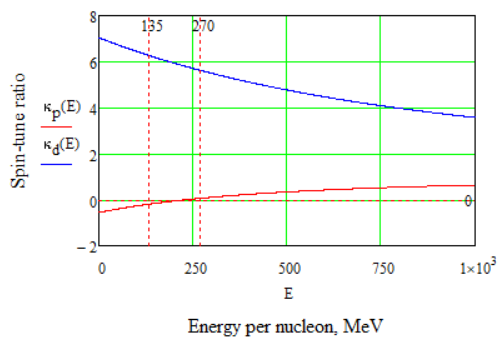
\includegraphics[width=0.55\linewidth]{4_spin-tune_ratio}
	\caption{Отношение спин-тюнов $\kappa = \cfrac{\nu_{\mathrm{B}_{\perp}}}{\nu_{\mathrm{E}}}$ поперечного магнитного и электрического поля для дейтрона и протона.}
	\label{fig:4_spin-tune}
\end{figure}

\par Эти фундаментальные различия накладывают конкретные требования на проектирование накопительного кольца для исследования обоих типов частиц. В частности, ур.~\ref{eq:deflection} показывает, что направление вращения спина протона и дейтрона различается, что требует либо смены полярности полей спинового компенсатора, либо его поворота на угол $\pi$ вокруг продольной оси. Кроме того, минимальная длина компенсатора, определяемая ур.~\ref{eq:length_min}, для протонов оказывается больше, чем для дейтронов при оптимальной энергии поляриметра. Это несоответствие может быть компенсировано снижением энергии протонов (рис. \ref{fig:4_ele_length}). При длине компенсатора, эквивалентной используемой для дейтронов, энергия протонов должна быть уменьшена до 73 МэВ, что приводит к снижению анализирующей способности примерно в 2–3 раза — достаточно для отработки методики, но недостаточно для получения статистически значимых результатов (табл. \ref{tab:particles}). Для создания дополнительных электромагнитных полей в роли спинового компенсатора рассматриваются два подхода: использование фильтра Вина или электростатического дефлектора с кикером, которые будут подробно обсуждены далее.

\begin{figure}[!h]
	\centering
	\includegraphics*[width=0.55\columnwidth]{4_total_length}
	\caption{Зависимость длины компенсирующего элемента в зависимости от энергии сгустка на нуклон.}
	\label{fig:4_ele_length}
\end{figure}

\begin{table}[!htb]

	\centering
	\caption{Параметры частиц, оптимальная энергия эксперимента и соответствующая полная длина спин компенсирующих элементов.}
	\label{tab:particles}
	\begin{tabular}{lccccc}
		\toprule
		Частицы & $A/Z$ & $G$     & $\gamma_{\text{exp}}$ & $E_{\text{exp}}$, МэВ/нуклон  & $L$, м \\
		\midrule
		Дейтрон $\text{d}$ & $2$   & $-0.14$ & $1.144$  & $135$ & $53$ \\
		Протон $\text{p}$ & $1$   & $1.79$  & $1.289$ & $270$ & $247$ \\
		&    &   & $1.078$ & $73$ & $53$ \\
		\bottomrule
	\end{tabular}
\end{table}

	\subsection{Применение прямого фильтра Вина со скрещенными полями}

\par Прямой Фильтр Вина представляет собой устройство в ускорителях частиц, предназначенное для управления спиновой динамикой без изменения орбитальной траектории пучка. Это достигается за счёт взаимной компенсации перпендикулярных магнитного и электрического полей. В такой конфигурации частицы движутся по прямой линии, одновременно подавляя эффект МДМ, что делает фильтр Вина полезным для экспериментов, требующих точного управления спином. Конструкция фильтра обеспечивает отсутствие отклонения вдоль линии пучка, минимизируя дополнительные требования к пространству на прямых участках кольца и сохраняя классическую последовательность расположения элементов.

\par На рис.~\ref{fig:wien-filter} представлены принципиальные схемы c квази-замороженным спином для дейтрона, так и для протона. Во-первых, показано, что отклонение спина за один период вследствие МДМ-эффекта в магнитной арке больше для протона. Во-вторых, направления полей для разных типов частиц противоположны.

\begin{figure} [h!]
	\centering
	а. Дейтрон\\
	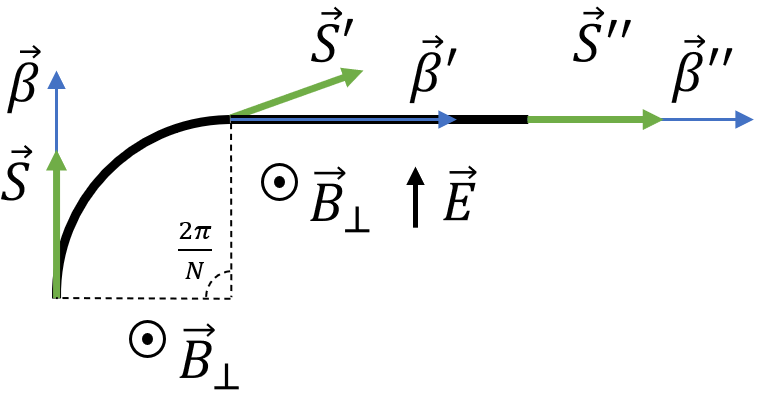
\includegraphics[width=0.6\linewidth]{4_wien-filter_deuteron}\\
	б. Протон\\
	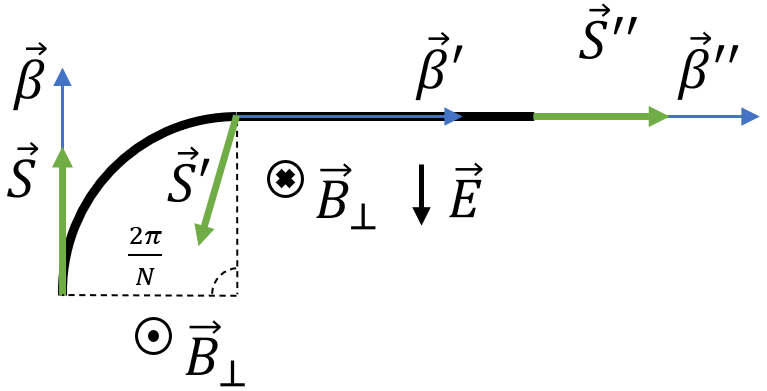
\includegraphics[width=0.6\linewidth]{4_wien-filter_proton}
	\caption{Принципиальная схема одного периода структуры с квази-замороженным спином с фильтрами Вина для а. дейтронов, б. протонов.}
	\label{fig:wien-filter}
\end{figure}

\par Адаптивность фильтра Вина заключается в возможности его применения как для дейтронов, так и для протонов. Для дейтронов фильтр применяется непосредственно на оптимальных энергиях, тогда как для протонов в той же структуре требуется изменить полярность полей или повернуть установку на $\pi$ вдоль продольной оси и использовать на более низких энергиях. Такая гибкость обеспечивает разработку методики изучения спиновой динамики различных типов частиц. В целом, способность фильтра управлять спином частиц без нарушения орбиты делает его перспективным элементом современных прецизионных экспериментов.

	\subsection{Применение электростатического дефлектора и дополнительного киккера}

\par Чисто электростатический дефлектор предназначен для изменения траекторий частиц и спиновой динамики за счёт создания радиального электрического поля с ненулевой кривизной. В отличие от фильтра Вина, дефлектор требует дополнительного киккера для компенсации орбитальных отклонений, что увеличивает общую длину спинового компенсатора.

\par При введении электростатической арки с кривизной $\Phi_{p\textrm{E}}^{\textrm{def}}$ магнитные арки должны дополнительно поворачивать на угол $\Phi_{p\textrm{B}}^{\textrm{kick}}$ с помощью киккеров. На рис.~\ref{fig:4_arc_B_E}а показано поведение спин-вектора дейтрона при последовательном действии магнитной арки, киккера, электростатической арки с отрицательной кривизной и симметрично расположенного киккера. Для протона изменяются кривизна электростатической арки и киккеров; при измерениях на полной энергии увеличивается их эффективная длина, что представлено на рис.~\ref{fig:4_arc_B_E}б. Поворот импульса после прохождения периода должен быть скорректирован на $\frac{2\pi}{N}$ для соблюдения квази-замороженного условия.

\begin{figure} [h!]
	\centering
	а. Дейтрон\\
	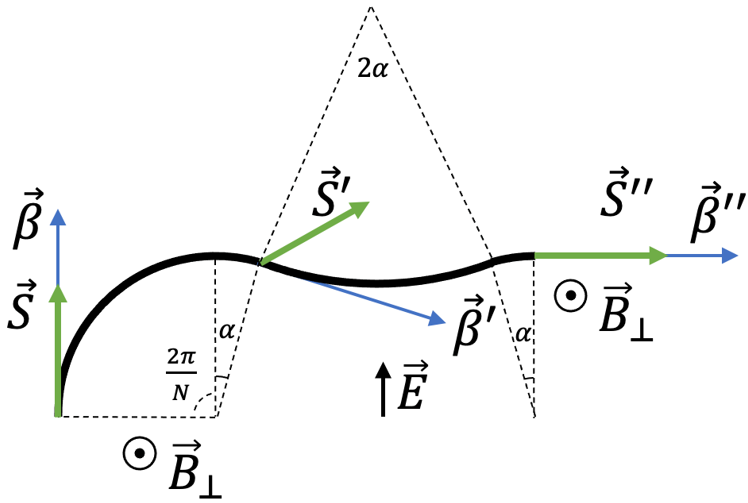
\includegraphics[width=0.6\columnwidth]{4_deflector_deutron}\\
	б. Протон\\
	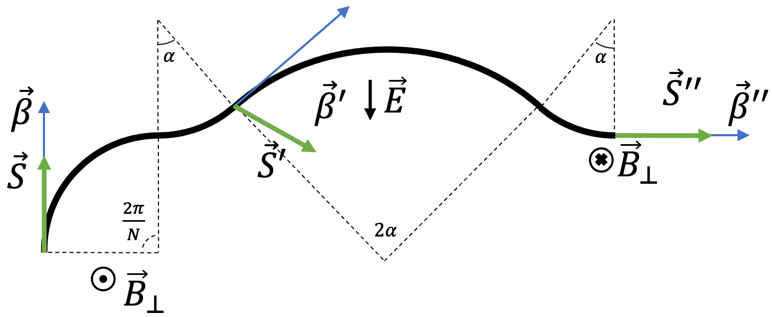
\includegraphics[width=0.77\linewidth]{4_deflector_proton}
	\caption{Принципиальная схема одного периода квази-замороженной структуры с электростатическими дефлекторами для а. дейтронов, б. протонов.}
	\label{fig:4_arc_B_E}
\end{figure}

\par Использование таких элементов актуально при создании обводных секций в дополнение к исходным прямым секциям, что позволяет варьировать конфигурацию установки. При этом необходимо учитывать пространственные зазоры между элементами для обеспечения независимой работы. Основная сложность заключается в том, что каждый тип частиц требует индивидуальной кривизны, определяемой на этапе проектирования структуры. Несмотря на это, электростатический дефлектор с киккером обеспечивает эффективное управление спином и траекторией частиц.
\newline
\par Данный результат показывает, что для реализации квази-замороженного спина принципиально важно наличие отклоняющих полей. При применении чисто электростатических дефлекторов требуется дополнительный внешний магнитный киккер, тогда как в случае фильтра Вина используются скрещенные магнитное и электростатическое поля, при этом интегральная величина поля сохраняется.

\par  Из рассмотренных принципиальных структур следует, что одновременное изучение ЭДМ дейтрона и протона возможно в в структуре с фильтрами Вина. Длина дефлекторов сопоставима с длиной фильтров Вина, однако при их применении требуются дополнительные киккеры, а кривизна для протонов и дейтронов имеет противоположный знак. Фильтры Вина располагаются на прямых участках, не требуют альтернативного канала, и для изучения протонов достаточно изменить полярность или повернуть элемент на $\pi$ относительно продольной оси. Применение дефлекторов оправдано в случаях, когда существует возможность естественного орбитального отклонения пучка для создания обводного канала.

	\section{Применение концепции квази-замороженного спина в действующих ускорительных установках}\label{sec:EDM/nuclotron}

\par Оптимальная энергия ЭДМ эксперимента составляет 270 МэВ, однако никаких ограничений относительно орбитального вращения в арке не сделано. Основным условием является обеспечение поворота импульса на угол $\Phi_p^{\textrm{arc}}$ с соответствующим поворотом спина на $\Phi_s^{\textrm{arc}}$, что достигается достаточным интегралом магнитного поля. Величина магнитного поля изменяется произвольно, однако её оптимальное значение с учётом особенностей структуры позволяет минимизировать эффективную длину поворотных арок. Такой подход не только оптимизирует эксперименты на текущем уровне энергии, но и обеспечивает работу с пучками при энергиях, потенциально достигающих нескольких ГэВ. Универсальность метода квази-замороженного спина позволяет интегрировать его в различные установки, включая существующие ускорительные кольца, с соблюдением требований к экспериментам на повышенных энергиях. Применение предложенного подхода рассмотрено для двух установок ОИЯИ: бустера Nuclotron для коллайдера NICA и самого коллайдера.

	\section{Использование Nuclotron в качестве бустера лёгких поляризованных частиц в коллайдер NICA}\label{sec:EDM/nuclotron}

\par Рассмотрим возможность использования синхротрона Nuclotron для ЭДМ исследований с применением концепции квази-замороженного спина.
\par В первом варианте предлагается сохранить текущие параметры ускорителя и одновременно создать условия для проведения экспериментов по измерению электрического дипольного момента дейтрона. Для этого на кольце устанавливаются электрические дефлекторы или фильтры Вина, обеспечивающие сохранение направления вектора спина вдоль пучка поляризованных частиц. Параметры Коллайдера, критическая энергия и характеристики электронного охладителя при этом остаются без изменений.

\par Во втором варианте предусматривается частичное изменение параметров для согласования с коллайдером. Энергия инжекции поляризованных протонов в коллайдер сохраняется на уровне 2–3 ГэВ. Чтобы избежать прохождения критической энергии после электронного охлаждения, планируется поднять критическую энергию в Коллайдере выше максимальной энергии эксперимента.

	\subsection{Требования к магнитооптической структуре синхротронов Nuclotron-NICA в задаче исследования ЭДМ лёгких ядер}\label{sec:EDM/requirements}

\par Текущая структура Nuclotron не предусматривает проведение экспериментов по измерению ЭДМ. Рассмотрим возможные способы реализации такой программы на существующей установке и потенциальные варианты её модернизации. В первую очередь необходимо определить ключевые требования с точки зрения спиновой динамики. Основным из них является компенсация вращения, обусловленного МДМ. Для этого может быть применён метод замороженного спина, при котором вектор спина остаётся сонаправленным с импульсом вдоль орбиты, а относительное МДМ-вращение отсутствует. Как следует из уравнения Т-БМТ и проведённого анализа, реализация этой схемы требует использования элементов со скрещёнными электрическим и магнитным полями. Применение чисто магнитных арок делает невозможным компенсацию МДМ-вращения методом замороженного спина.

\par В качестве альтернативы методу замороженного спина может быть использован метод квази-замороженного спина, основанный на пространственном разделении электрического и магнитного полей с последующей компенсацией МДМ-компоненты. Компенсация осуществляется на прямых участках с использованием электрического поля. В качестве компенсирующих элементов могут применяться электростатические дефлекторы или фильтры Вина со скрещёнными электрическим и магнитным полями.

\par Следует подчеркнуть, что Nuclotron планируется использовать в качестве бустера для коллайдера NICA. Поэтому наряду с низкоэнергетической опцией, предназначенной для проведения ЭДМ-экспериментов при энергии порядка сотен МэВ, необходимо обеспечить возможность ускорения поляризованного протонного пучка до энергий порядка нескольких ГэВ. В этих условиях основную роль в процессе ускорения должно играть магнитное поле поворотных диполей, поскольку применение электрического поля для достижения таких энергий нецелесообразно. При этом критическая энергия установки должна находиться выше максимальной энергии пучка.
	
	\subsection{Текущая магнитооптика Nuclotron}\label{sec:EDM/optics}
\par Принципиальная схема текущей восьмипериодической структуры Nuclotron с длиной $L_{\text{NUC}}=251$ м представлена на рис. \ref{fig:4_Nuclotron_original}а. На рис.~\ref{fig:4_old_nuclotron} изображены параметры Твисса для одного периода, неоптимальные с точки зрения подавления дисперсионной функции на прямых участках. Суммарная длина прямых промежутков составляет $L_{\text{free}} = 7\times8=56$ м. Следовательно, размещение фильтров Вина с длиной $L_{\text{WF}} = 53$ м на прямых участках немодернизированной структуры Nuclotron практически полностью исключает возможность установки дополнительного необходимого оборудования. 

\par Рассмотрим возможность создания обводных каналов в исходной структуре. В качестве компенсирующих элементов предполагаются электростатические дефлекторы, обладающие ненулевым радиусом кривизны. При таком подходе оборудование можно расположить параллельно при наличии достаточного расстояния между полученными каналами. На рис. \ref{fig:4_Nuclotron_original}б показана принципиальная схема текущей структуры Nuclotron с электростатическими дефлекторами. Максимальное расстояние между каналами может составить порядка $18$ см, что недостаточно для параллельного расположения.

\begin{figure}[!h]
	\centering
	а.\includegraphics*[width=0.47\columnwidth]{4_Nuclotron_original.png}
	б.\includegraphics*[width=0.47\columnwidth]{4_Nuclotron_original_def.png}
	\caption{Принципиальная схема расстановки структуры Nuclotron с текущим расположением элементов и с введением электростатических дефлекторов.}
	\label{fig:4_Nuclotron_original}
\end{figure}

\begin{figure}[!h]
  \centering
	\includegraphics*[width=0.99\columnwidth]{4_old_nuclotron}
   \caption{Твисс-функции текущей регулярной структуры Nuclotron.}
   \label{fig:4_old_nuclotron}
\end{figure}

\par Приведённые факты показывают необходимость увеличения длины прямых участков. Может быть рассмотрена модернизация структура с оптимизированными диполями с максимальным магнитным полем $1.8$ Тл. Суммарная длина прямых промежутков должна составить $L_{\text{free}}+L_{\text{WF}}=56+53 = 109$ м. Оставшееся место будет использовано для расстановки магнитных элементов: диполей, квадруполей, секступолей. Длина магнитной арки $L_{\textrm{arc}}=17.5$ м, а длина магнитов изменяется от $1.44$ м до $1.78$ м, при этом их количество сокращается вдвое с $96$ до $48$. Тогда максимальная энергия протонного пучка может составлять до $6.5$ ГэВ. Данная опция удовлетворяет требованию использования Nuclotron в качестве бустера при $2-3$ ГэВ, а также возможности его использования на выведенной мишени экспериментов BM@N c понижением энергии с $10$ ГэВ до $6.5$~ГэВ \cite{kovalenko:nuclotron}. Фильтры Вина могут быть расположены на прямых участках, а для дефлекторов неизбежно должны быть реализованы дополнительные каналы.

	\subsection{Модернизированная восьмипериодическая структура}\label{sec:EDM/optics/8period}

\par Реализована восьмипериодическая структура на основе простейшей ФОДО ячейки. В такой конфигурации возможно применение обеих опций компенсации МДМ-компоненты: с использованием прямых фильтров Вина либо электростатических дефлекторов в сочетании с киккер-магнитами. В случае применения дефлектров отсутствует необходимость использования прямых промежутков для ЭДМ эксперимента. Размещение дефлекторов может осуществляться как по краям, так и в центральной части каналов, что показано на рис. \ref{fig:4_Nuclotron_8}. Расстояние между каналами составляет $47$ и $50$~см соответственно.

\par Подавление дисперсии на арке может быть осуществлено выбором кратного количества набега фазы $\nu_{x,y} = 1$, что показано на рис. \ref{fig:4_Nuclotron_8}. Стоит отметить, что наличие электростатических элементов при энергии $E_{\textrm{edm}}=270$ МэВ приводит к искажению дисперсии на длине периода, без возможности компенсации соответствующим магнитным полем. Однако, она может быть дополнительно компенсирована квадруполями арки, при этом набег фазы также искажается, что может приводить к сложностям с подавлением нелинейности. Пример такой компенсации показан на рис.~\ref{fig:4_Nuclotron_twiss_8}.

\begin{figure}[!h]
  \centering
   a.\includegraphics*[width=0.47\columnwidth]{4_Nuclotron_8_def2.png}
   б.\includegraphics*[width=0.47\columnwidth]{4_Nuclotron_8_def1.png}
   \caption{Принципиальная схема восьмипериодической структуры Nuclotron с текущей расстановкой при введении электростатических дефлекторов.}
   \label{fig:4_Nuclotron_8}
\end{figure}

\begin{figure}[!h]
  \centering
   \includegraphics*[width=1\columnwidth]{4_Nuclotron_twiss_8}
   \caption{Твисс-функции регулярной поворотной арки восьмипериодической модернизированной структуры Nuclotron.}
   \label{fig:4_Nuclotron_twiss_8}
\end{figure}

\begin{figure}[!h]
  \centering
   \includegraphics*[width=1\columnwidth]{4_Nuclotron_Def_twiss_8}
   \caption{Твисс-функции регулярной поворотной арки восьмипериодической модернизированной структуры Nuclotron с дефлекторами.}
   \label{fig:4_Nuclotron_Def_twiss_8}
\end{figure}

\newpage
	\subsection{Модернизированная 16-периодическая структура}\label{sec:EDM/optics/16period}

\begin{figure}[!h]
  \centering
   \includegraphics*[width=0.5\columnwidth]{4_Nuclotron_16.png}
   \caption{Принципиальная схема 16-ти периодической структуры Nuclotron с текущей расстановкой при введении фильтров Вина.}
   \label{fig:4_Nuclotron_16}
\end{figure}

\begin{figure}[!h]
  \centering
   \includegraphics*[width=1\columnwidth]{4_Nuclotron_twiss_16.png}
   \caption{Твисс-функции 16-периодической модернизированной структуры Nuclotron без фильтров Вина.}
   \label{fig:4_Nuclotron_twiss_16}
\end{figure}

\begin{figure}[!h]
  \centering
   \includegraphics*[width=1\columnwidth]{4_Nuclotron_WF_twiss_16.png}
   \caption{Твисс-функции 16-периодической модернизированной структуры Nuclotron c фильтрами Вина.}
   \label{fig:4_Nuclotron_twiss_16_WF}
\end{figure}

\par Увеличение числа периодов структуры с квази-замороженным спином позволяет приблизить ее свойства к характерным для режима замороженного спина и, как следствие, повысить точность проведения эксперимента. Периодичность структуры особенно значима для излучения ЭДМ протона, что отражено в табл. \ref{tab:edm}. Для изменения числа периодов, в уже рассмотренной восьмипериодической структуре, магнитная арка может быть раздвинута для создания дополнительного прямого промежутка. Принципиальная схема показана на рис.~\ref{fig:4_Nuclotron_16}, а конкретная магнитооптика без фильтров Вина на рис.~\ref{fig:4_Nuclotron_twiss_16} и с фильтрами Вина на рис.~\ref{fig:4_Nuclotron_twiss_16_WF}. Такой подход нарушает регулярность и соответствующая структура должна быть рассмотрена как резонансная, подобно представленному в Главе \ref{ch:resonant}. Стоит отметить, что данная структура называется 16-периодической по причине возможности разделения фильтров Вина на большее количество, уменьшая угол отклонения спин-вектора вдвое относительно приведенной выше структуры. Однако, по своей сути, магнитная структура имеет периодичность равную восьми.

\par При проектировании магнитооптической структуры модернизированного Nuclotron преследовались несколько ключевых целей. Во-первых, суперпериод сформирован таким образом, чтобы центральная ячейка содержала дрейфовый участок без поворотных магнитов в точке максимального значения дисперсионной функции при бесконечной кривизне траектории, что обеспечивает повышение критической энергии. Во-вторых, число суперпериодов, равное восьми, лишь незначительно превышает горизонтальную бетатронную частоту ${\nu}_x$, что упрощает регулировку коэффициента уплотнения орбиты и, как следствие, контроль критической энергии. В-третьих, наличие центрального дрейфа упрощает размещение трёх семейств секступолей, необходимых для компенсации бетатронной и спиновой хроматичностей, а боковые дрейфовые участки обеспечивают удобное размещение фильтров Вина.

\par Рассмотренные модернизированные структуры Nuclotron приведены в табл.~\ref{tab:structures}.

\begin{table}[!htb]
	\centering
	\caption{Основные параметры модернизированных структур Nuclotron.}
	\label{tab:structures}
	\begin{tabular}{|>{\raggedright\arraybackslash}p{2.7cm}|c|c|c|c|c|}
		\hline
		Структура & \makecell[c]{Длина \\ магнита, м} & \makecell[c]{Количество \\ магнитов} & \makecell[c]{$B\rho$, \\ Т$\cdot$м} & \makecell[c]{Макс. энергия \\ дейтронов, ГэВ} & \makecell[c]{Макс. энергия \\ протонов, ГэВ} \\
		\hline
		Текущая & 1.44 & 96 & 39.6 & 10.14 & 10.97 \\
		\hline
		8-период. & 1.78 & 48 & 24.4 & 5.7 & 6.47 \\
		\hline
		16-период. & 1.78 & 48 & 24.5 & 5.7 & 6.47 \\
		\hline
	\end{tabular}
\end{table}

	\section{Предпосылки модернизации главного кольца NICA}\label{sec:EDM/Wien_filter/modernization}

\par Для исследования ЭДМ в кольце коллайдера NICA применяется концепция квази-замороженного спина, что обусловлено использованием чисто магнитных поворотных арок. В коллайдерной конфигурации пространство прямых участков занято необходимым оборудованием (охлаждение, ускоряющие ВЧ-станции, диагностика), а также присутствуют точки соударения для проведения экспериментов в детекторах. Для решения указанных ограничений могут быть созданы альтернативные обводные каналы (bypass) с установкой прямых фильтров Вина. Это обеспечивает возможность использования главного кольца NICA в режиме накопителя, а не только коллайдера, без значительной перестройки комплекса и дополнительных затрат, расширяя спектр доступных экспериментов. Коллайдер имеет форму рейстрека (racetrack) с двумя магнитными поворотными арками и периодичностью $N=2$. Такая конфигурация ограничивает потенциал накопления ЭДМ-компоненты для протонов, сохраняя при этом возможность исследования ЭДМ дейтронов. Дополнительным преимуществом является наличие двух колец, что позволяет проводить эксперименты с пучком в прямом и обратном направлениях.

\par При проектировании накопительного кольца NICA с обводными каналами необходимо оставить геометрию арок неизменной для полного сохранения исходных функций. Остается возможным только изменение полей в уже установленных элементах. В будущем вся предлагаемая магнитооптика будет рассмотрена для дейтронов с энергией $240$~МэВ. Стоит отметить, что расчеты показывают основные параметры магнитного поля основных диполей арки $B_{\textrm{dip}}=0.132$~Тл, а также магнитную жесткость $B\rho=3.252 \ \textrm{Тл} \cdot$м. Ненулевая дисперсия в поворотной арке подавлена по её краям. Таким образом, прямой участок имеет нулевую дисперсию по всему периметру. Общая длина оригинального кольца NICA $L_{\textrm{acc}}~=~503.04$~м, длина одной арки составляет $L_{\textrm{arc}}~=~142.15$~м, следовательно, остаётся доступным $\left(L_{\textrm{acc}}-2L_{\textrm{arc}}\right)/2~=~109.6$~м для организации обводного канала.

\par Для орбитального отклонения рассматривались дипольные магниты, чтобы обеспечить поворот на угол $\alpha=\ 9^{\circ}$. Сила диполя $B_{\textrm{BP}}=1$~Тл при длине $L_{\textrm{dip}}^{\textrm{BP}}=50$~см. Альтернативный прямой участок находится на расстоянии $1$ м от исходного, поэтому длина обводного участка $L_{\textrm{BP}}=1\mathrm{м/sin\alpha}\sim6.4$ м. Принципиальная схема обходных каналов показана на рис. \ref{fig:4_NICA_bypass}.

\begin{figure}[!h]
  \centering
   \includegraphics*[width=1.0\columnwidth]{4_NICA_bypass.png}
   \caption{Принципиальная схема обводных каналов bypass в существующем комплексе NICA.}
   \label{fig:4_NICA_bypass}
\end{figure}

\par Отклоняющие магниты искажают дисперсионную функцию. Таким образом, было необходимо использовать по меньшей мере 2 фокусирующих квадруполя на обводном канале для подавления дисперсии на выходе. Это поможет обеспечить нулевую дисперсию на всем прямолинейном участке. Чтобы гарантировать периодичность и симметрию бета-функций, можно использовать один, либо три дефокусирующих квадруполя. Будут рассмотрены два случая, с адаптированными прямыми участками, состоящими из ФОДО ячеек. Это сделано для простоты моделирования в регулярной идеальной структуре. Наконец, мы рассмотрим реальный случай магнитооптики.

	\subsection{Первичная схема с 3 квадруполями}\label{sec:EDM/Wien_filter/ByPass/3quad}

\begin{figure}[!h]
	\centering
	\includegraphics*[width=1.0\columnwidth]{4_bypass_3scheme.png}
	\caption{Принципиальная схема bypass с 3 квадруполями.}
	\label{fig:4_bypass_3scheme}
\end{figure}

\par В приведённом случае отклоняющая секция состоит из минимально возможных 3 квадруполей: 2 фокусирующих QBP1 и 1 дефокусирующий QBP2. Согласование арки обеспечивается тремя квадруполями QM1, QM2, QM3 (секция согласователя Matching M1). Согласование отклоняющей секции с прямым участком симметрично осуществляется такими же квадруполями QM1, QM2, QM3. Принципиальная схема показана на рис.~\ref{fig:4_bypass_3scheme}. Это возможно в силу изначально заложенной симметрии между аркой и прямым участком. Тогда общая длина всего ускорителя составит $L_{\textrm{3quad}}^{\textrm{acc}}=503.46$~м.
\par На рисунке \ref{fig:4_bypass_3quad} приведены Твисс-функции, черными линиями указаны границы отклоняющего участка. Максимум бета-функции $\beta_y$ расположен в центре канала и может принимать большее значение, по сравнению с $\beta_{x}$. По этой причине можно рассмотреть случай с 5 квадруполями в обводном канале.

\begin{figure}[!h]
  \centering
   \includegraphics*[width=1.0\columnwidth]{4_bypass_3quad}
   \caption{Твисс-параметры для bypass с 3 квадруполями. Черными линиями показано расположение дефлекторов.}
   \label{fig:4_bypass_3quad}
\end{figure}

	\subsection{Модернизированная схема с 5 квадруполями}\label{sec:EDM/Wien_filter/ByPass/5quad}

\par По сравнению с рассмотренным случаем, отклоняющий канал состоит из 5 квадруполей, которые представлены 2 семействами: фокусирующим QBP1 и дефокусирующим QBP2. Он становится длиннее $L_{\textrm{5quad}}^{\textrm{BP}}=9.35$~м и отклоняется на $1.46$~м., что показано на рис.~\ref{fig:4_bypass_5scheme}. Теперь секции согласования M1 и M2 по-прежнему идентичны, но представлены двумя квадруполями QM1 и QM2 для обеспечения регулярности Твисс-функций. Однако, полная длина ускорителя становится больше исходного $L_{\textrm{5quad}}^{\textrm{acc}}=510.02$~м. На рис.~\ref{fig:4_bypass_5quad} показано, что максимум $\beta_y$ становится меньше в центре. Стоит отметить, что максимум дисперсионной функции стал увеличился от $D_x^{\textrm{3quad}} \sim 0.2$ м до $D_x^{\textrm{5quad}} \sim 0.5$ м. Таким образом, этот случай должен быть адаптирован к реальному.

\begin{figure}[!h]
  \centering
   \includegraphics*[width=1.0\columnwidth]{4_bypass_5scheme.png}
   \caption{Принципиальная схема bypass с 5 квадруполями.}
   \label{fig:4_bypass_5scheme}
\end{figure}

\begin{figure}[!h]
  \centering
   \includegraphics*[width=1.0\columnwidth]{4_bypass_5quad}
   \caption{Твисс-параметры для bypass с 5 квадруполями. Черными линиями показано расположение дефлекторов.}
   \label{fig:4_bypass_5quad}
\end{figure}

	\subsection{Адаптированный вариант}\label{sec:EDM/Wien_filter/ByPass/final}

\par Основываясь на рассмотренных примерах можно, наконец, получить максимально адаптированную к реальным длинам установки структуру. Теперь рассмотрим полностью регулярный прямой участок, который стал короче $L_{\textrm{SS}}^{\textrm{BP}}=80.71$ м (рис. \ref{fig:4_bypass_real_scheme}). Отклоняющий канал состоит из 5 квадруполей и отклоняет пучок на $1.46$ м. Однако, для согласования использовались разные секции M1 и M2, чтобы компенсировать асимметрию между поворотной аркой и прямым участком. Наконец, твисс-функция половины bypass NICA, представлена на рис.~\ref{fig:4_bypass_twiss_ring}. В центре прямой секции расположены фильтры Вина. Все расчеты выполнены при помощи программ OptiM \cite{optim} и COSY Infinity \cite{cosy}.

\begin{figure}[!h]
  \centering
   \includegraphics*[width=1.0\columnwidth]{4_bypass_real_scheme.png}
   \caption{Принципиальная схема адаптированной структуры кольца NICA c bypass.}
   \label{fig:4_bypass_real_scheme}
\end{figure}

\begin{figure}[!h]
  \centering
   \includegraphics*[width=1.0\columnwidth]{4_bypass_twiss_ring.png}
   \caption{Твисс-функции для половины адаптированной структуры кольца NICA c bypass. Фильтры Вина, расположенные на прямом участке.}
   \label{fig:4_bypass_twiss_ring}
\end{figure}

\newpage
	
	\section{Cпин-орбитальный трекинг в магнитном кольце со скрещенными E+B элементами} \label{sec:EDM/Wien_filter_tracking}

\par Траектория спина показана на рис. \ref{fig:4bypassspin} в одной половине модернизированного кольца bypass NICA и состоит из: поворотной арки, отклоняющего канала, прямого сегмента и двух секций согласователя (M1 и M2). Рассматривается вертикально поляризованная частица с небольшим начальным отклонением. Как видно, фильтры Вина на прямом участке компенсируют вращение спина в арке и восстанавливают его до исходного значения.

\begin{figure}[!h]
	\centering
	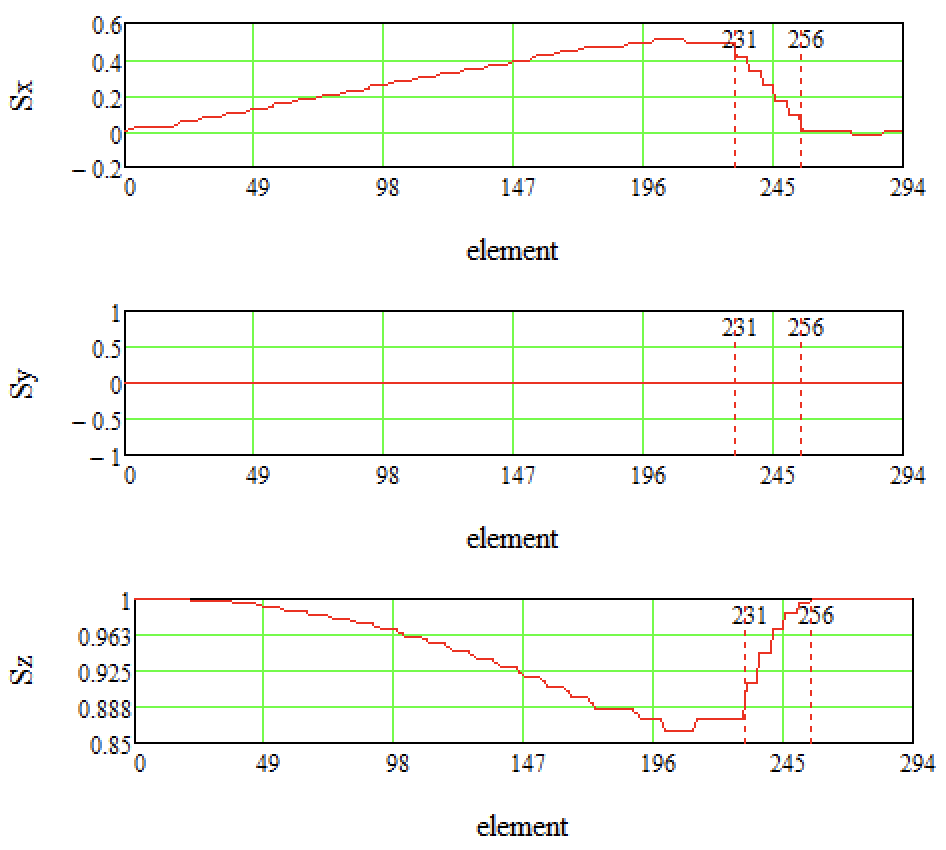
\includegraphics[width=0.7\linewidth]{images/4_bypass_spin}
	\caption{Траектория спина в половине модернизированного кольца bypass NICA. Арка и прямая секция с фильтрами Вина (границы обозначены красными пунктирными линиями). Вертикально поляризованная частица $\vec{S}~(0,0,1)$. Показана зависимость $S_{x}$, $S_{y}$ и $S_{z}$ от номера элемента (длины).}
	\label{fig:4bypassspin}
\end{figure}

\par Орбитальное движение частиц в трехмерном пространстве оказывает влияние на спиновую динамику, и, согласно ур.~\ref{eq:T-BMT}, спин различных частиц, прецессирует с отличными частотами вокруг инвариантной оси. При значительном разбросе нарушается спиновая когерентность, тем самым ограничивая возможность измерения ЭДМ. Для обеспечения спиновой когерентности необходимо использовать нелинейные элементы, секступоли, расположенные в местах с ненулевой дисперсией, на поворотных арках. Так как секступоли также влияют и на бетатронную хроматичность, мы рассматриваем возможность одновременного подавления обоих эффектов.

		\subsection{Декогеренция спина}\label{sec:EDM/Wien_filter_tracking/decoherence}

\par Сдвиг распределения равновесного уровня энергии из-за бетатронного движения и ненулевого коэффициента уплотнения импульса второго порядка основан на синхронном принципе \cite{Senichev:2013_decoherence} и определяется с помощью:

\begin{equation}
\Delta\delta_{eq}=\frac{\gamma_s^2}{\gamma_s^2\alpha_0-1}\left[\frac{\delta_0^2}{2}\left(\alpha_1+\frac{3}{2}\frac{\beta_s^2}{\gamma_s^2}-\frac{\alpha_0}{\gamma_s^2}+\frac{1}{\gamma_s^4}\right)+\left(\frac{\Delta L}{L}\right)_\beta\right].
\label{eq:equilibrium}
\end{equation}

\noindent Для определения относительного удлинения орбиты из-за бетатронных колебаний:

\begin{equation}
\left(\frac{\Delta L}{L}\right)_\beta=\frac{\pi}{2L}\left[\epsilon_x\nu_x+\epsilon_y\nu_y\right],
\end{equation}

\noindent где индекс $s$ означает синхронную частицу, $\epsilon_x$, $\epsilon_y$ – эмиттансы, $\nu_x$, $\nu_y$ – частота бетатронных колебаний, $\delta_0$ – относительный разброс импульса, $\alpha_0$, $\alpha_1$ – два первых порядка коэффициента уплотнения импульса. Разные частицы имеют различный импульс, и существует необходимость в использовании понятия эффективной энергии пучка:

\begin{equation}
	\gamma_{\text{eff}}=\gamma_s+\beta_s^2\gamma_s\Delta\delta_{eq}.
\end{equation}

\par Разброс по энергии происходит вследствие удлинения орбиты \cite{orbit_length}:

\begin{equation}
\frac{\Delta C_\Sigma}{C_{0}}
=-2\pi\left(J_x\xi_x+J_y\xi_y\right)+\delta_0\left(\alpha_0+\alpha_1\delta_0+\alpha_2\delta_0^2+\ldots\right),
\label{eq:orbit_length}
\end{equation}

\noindent где $\xi_x$, $\xi_y$ – хроматичность в $x, y$ плоскостях. Исходя из представленных уравнений, для коррекции орбитального движения могут быть использованы секступоли для компенсации натуральной хроматичности, а также коэффициента уплотнения орбиты.

		\subsection{Секступольная коррекция}\label{sec:EDM/Wien_filter_tracking/sextupole_correction}

\par Достижение спиновой когерентности является отдельной сложной задачей, и такие эксперименты были проведены на ускорителе COSY в Юлихе, Германия, чтобы получить время когерентности (Spin Coherence Time) SCT на уровне $1000$ с \cite{1000}. Секступоли располагаются в местах с ненулевой дисперсией на поворотных арках. В минимумах и максимумах дисперсионной $D_{x,y}$ и бета $\beta_{x,y}$ функциях оказывают наибольшее воздействие и физически располагаются рядом с квадрупольными линзами. Твисс-функции арки NICA являются регулярными и показаны на рис. \ref{fig:4_NICA_arc}.

\begin{figure}[!h]
  \centering
   \includegraphics*[width=1.0\columnwidth]{4_NICA_arc.png}
   \caption{Твисс-параметры bypass NICA для дейтронного режима в OptiM. Также показано расположение секступольных семейств.}
   \label{fig:4_NICA_arc}
\end{figure}

\par Для коррекции бетатронной хроматичности достаточно использовать только 2 семейства секступолей: одно вблизи фокусирующих квадруполей, другое – рядом с дефокусирующими. Натуральная хроматичность рассматриваемого накопительного кольца bypass NICA равна $\nu_{x,y}=-17/-17$. Рис. \ref{fig:4_spin_dependance}  изображает частоту прецессии спина после проведения оптимизации (красная линия показывает натуральную хроматичность, синяя – скорректированную, подавленную до нуля). Для этого случая также был осуществлен спин-трекинг в течение $3\times{10}^6$ оборотов для частиц с различным начальным отклонением в координатах $x, y, d$ с начальной ориентацией спина ${\vec{S}}_0$ под углом $45$ градусов в плоскости $y-z$, что показано на рис. \ref{fig:4_spin_decoherence}.

\begin{figure}[!h]
	\centering
	\includegraphics*[width=0.32\columnwidth]{4_spin_dependance_x.png}
	\includegraphics*[width=0.32\columnwidth]{4_spin_dependance_y.png}
	\includegraphics*[width=0.32\columnwidth]{4_spin_dependance_d.png}
	\caption{Зависимость частоты прецессии спина от координат x, y, d для различных случаев оптимизации. NC – натуральная хроматичность (красная линия); BC – нулевая (бетатронная) хроматичность (синяя пунктирная линия); SC – спиновая когерентность (зеленая линия); $BC_{\alpha}$ – нулевая хроматичность и $\alpha_1=0$ (фиолетовая линия); $BC_{\text{eta}}$ – нулевая хроматичность и ноль $\eta_1=0$ (светло-голубая линия).}
	\label{fig:4_spin_dependance}
\end{figure}

\begin{figure}[!h]
  \centering
   \includegraphics*[width=0.7\columnwidth]{4_spin_decoherence.png}
   \caption{Спиновый трекинг частиц с различным начальным отклонением в координатах x, y, d с использованием 2 семейств секступолей для получения нулевой бетатронной хроматичности.}
   \label{fig:4_spin_decoherence}
\end{figure}

\par С целью достижения спиновой когерентности перейдем к рассмотрению частоты прецессии спина. COSY Infinity \cite{cosy} не может работать вблизи нулевого значения частоты прецессии спина. Так как это может привести к ошибке из-за резонанса, необходимо произвести отстройку до уровня $\nu_s\sim{10}^{-4}$. Однако, нужно учитывать, что к частицам предъявляется требование синхронной прецессии. Основным параметром является частота вращения спина, которая в общем случае зависит от координат и энергии. Можно видеть, что доминирующим компонентом является квадратичный член в разложении частоты спиновой прецессии. Это видно на рис. \ref{fig:4_spin_dependance} для обоих случаев – как для натуральной хроматичности, так и скорректированной хроматичности. По этой причине секступоли могут быть выбраны другим способом, чтобы достичь спиновой когерентности, путем подавления вторых порядков.

\par Из ур.~\ref{eq:equilibrium}, \ref{eq:orbit_length} следует, что применение двух линейно независимых семейств секступолей является недостаточным для независимой вариации трех параметров орбитального движения. Таким образом, возникает необходимость использования третьего семейства для подавления зависимости от энергетической компоненты. Однако, в регулярных структурах $\beta$-функция и дисперсия не позволяют использовать 3 линейно независимых семейства. Введение линейно-зависимых семейств SF1, SF2, SD показано на параметрах Твисса. В этом методе мы не влияем на хроматичность, просто отслеживаем её значение $\nu_{x,y}=-13/-18$. Этого недостаточно для обеспечения стабильного орбитального движения. Тем не менее, приведенный случай показывает достижение спиновой когерентности, нет зависимости частоты спиновой прецессии от координат и энергии (рис.~\ref{fig:4_spin_dependance}: зеленая линия). Результаты спинового трекинга частиц подтверждают это утверждение. На рис.~\ref{fig:4_spin_coherence}, частота вращения спина~$\nu_s~\sim~{10}^{-7}$,~количество оборотов $3\times{10}^6$ или $3$ с. Частицы с различным начальным отклонением прецессируют с одинаковой спиновой частотой. Однако, в этом случае градиент секступольного поля принимает большое значение, что может вызвать нелинейные эффекты (табл.~\ref{tab:coherence}).

\begin{figure}[!h]
  \centering
   \includegraphics*[width=0.7\columnwidth]{4_spin_coherence.png}
   \caption{Спиновый трекинг частиц с различным начальным отклонением в координатах x, y, d с использованием 3-х семейств секступолей для получения спиновой когерентности.}
   \label{fig:4_spin_coherence}
\end{figure}

\begin{table}[!hb]
	\centering
	\caption{Сравнение параметров с различной вариацией оптимизации оптимизацией.}
	\begin{tabular}{|p{2.6cm}|m{2.5cm}|m{2.5cm}|m{2.5cm}|m{2.5cm}|m{2.5cm}|}
		\hline
		Параметр & Без оптимизации & Хро\-ма\-тич\-ность & Спиновая когерентность & Хро\-ма\-тич\-ность + $\alpha_1$ & Хро\-ма\-тич\-ность + $\eta_1$ \\
		\hline
		Значение хроматичности & -17/-17 & 0/0 & -13/-18 & 0/0 & 0/0 \\
		\hline
		Коэф. $\alpha_1$ & 0.2 & -0.4 & $-0.37 \times 10^{-2}$ & $\sim -10^{-12}$ & -0.85 \\
		\hline
		Коэф. $\abs{K_x}$ & $0.16 \times 10^{-1}$ & $0.55 \times 10^{-1}$ & $0.27 \times 10^{-13}$ & $0.55 \times 10^{-1}$ & $0.56 \times 10^{-1}$ \\
		\hline
		Коэф. $\abs{K_y}$ & $0.51 \times 10^{-2}$ & $0.76 \times 10^{-1}$ & $0.12 \times 10^{-12}$ & $0.78 \times 10^{-1}$ & $0.78 \times 10^{-1}$ \\
		\hline
		Коэф. $\abs{K_z}$ & $0.43 \times 10^{-1}$ & $0.20 \times 10^{-1}$ & $0.13 \times 10^{-12}$ & $0.13 \times 10^{-1}$ & $1.6 \times 10^{-1}$ \\
		\hline
		\# семейств секступолей & Без секступолей & 2 & 3 & 3 & 3 \\
		\hline
		Макс. поле секступолей [m$^{-3}$] & - & 2.7 & 19.4 & 4.9 & 104.2 \\
		\hline
	\end{tabular}
	\label{tab:coherence}
\end{table}

		\subsection{Коррекция высших порядков}\label{sec:EDM/Wien_filter_tracking/correction}

\par Как мы можем видеть, чистая коррекция бетатронной хроматичности не позволила получить нулевой разброс частоты вращения спина. Одновременно, достижение спиновой когерентности путем подавления квадратичного члена частоты спиновой прецессии не подавляет хроматичность. Исходя из ур. \ref{eq:orbit_length}, значение $\delta_0\alpha_0$ может быть усреднено с использованием ВЧ для смешивания. Таким образом, чтобы гарантировать нулевое удлинение орбиты, необходимо подавить горизонтальную и вертикальную хроматичность $\xi_x,\xi_y$ вместе со значением $\alpha_0$ до нуля. Это также возможно при использовании только независимых 3-х семейств секступолей. Представленный способ не позволяет добиться спиновой когерентности в рассматриваемой структуре. На рис. \ref{fig:4_spin_dependance} (фиолетовая линия) показана ненулевая зависимость частоты прецессии спина от координат. Аналогичное справедливо, если мы следуем ур. \ref{eq:equilibrium} и подавляем значение $\eta_1$ вместе с коррекцией хроматичности (рис. \ref{fig:4_spin_dependance} светло-синяя линия). Кроме того, максимальное значение секступольного градиента слишком велико и не может быть реализовано.

\par Окончательно, были рассмотрены различные случаи оптимизации секступолями. Квадратичные члены в разложении по частоте спиновой прецессии являются наиболее важными и представляют зависимость от координат и энергии. Все основные параметры, которые подвергались мониторингу, приведены в табл.~\ref{tab:coherence}. Согласно результатам проведенного исследования, одновременное достижение как бетатронной хроматичности, так и спиновой когерентности  является невозможным в случае применения трех семейств секступолей в регулярной структуре. Более того, максимальное значение коэффициента секступолей неудовлетворительно и может привести к нелинейным неустойчивостям. Стоит отметить, что регулярная дисперсионная функция на поворотной арке не позволяет найти три линейных независимых семейства, в силу их расположения в одних и тех же минимумах/максимумах $\beta$-функции, дисперсии $D$. Однако, дисперсионная функция может быть промодулирована таким образом, чтобы получить в чистом виде три линейных независимых семейства секступолей. Также одним из возможных решений проблемы является использование охлажденного пучка на уровне $\frac{dp}{p}\approx{10}^{-5}$, что может помочь свести к минимуму $\gamma$–эффективное и, наконец, обеспечить спиновую когерентность одновременно с подавленной бетатронной хроматичностью.

	\section*{Выводы}
\par Рассмотрена спин-орбитальная динамика элементарных частиц в синхротронах, функционирующих в режиме накопительного кольца. 

\begin{enumerate}

\item Исследована спиновая динамика в электрических и магнитных полях. Изучено поведение спина в электростатических дефлекторах, а также фильтрах Вина для реализации квази-замороженного спина;

\item Рассмотрены варианты модернизации кольца для проведения независимых ЭДМ-экспериментов с сохранением функции бустера. Предложены 8-ми и 16-ти периодические структуры с реализованной концепцией квази-замороженного спина. Наибольшие преимущества демонстрирует структура с использованием фильтров Вина, применимая для исследований ЭДМ как дейтронов, так и протонов при меньшей энергии;

\item Метод создания обводных каналов (bypass) позволяет формировать альтернативные прямые участки, расширяя область применения синхротрона для прецизионных фундаментальных экспериментов; 

\item Исследована возможность формирования когерентного пучка в регулярной структуре, что является необходимым условием применения метода частотной области при изучении ЭДМ. Подавление хроматичности и достижение когерентности с применением лишь двух семейств секступолей оказываются невозможными. Для этого требуется как минимум три независимых семейства, расположенных в максимумах бета- и дисперсионных функций. Реализация такого подхода связана с внесением нерегулярности в структуру, что, например, может быть достигнуто в резонансной структуре.

\end{enumerate}

\FloatBarrier
